\documentclass[aspectratio=1610]{beamer}
% \documentclass[aspectratio=1610,handout]{beamer}

\usetheme[%pageofpages=of,% String used between the current page and the
                         % total page count.
          bullet=circle,% Use circles instead of squares for bullets.
          titleline=true,% Show a line below the frame title.
          alternativetitlepage=true,% Use the fancy title page.
          titlepagelogo=figures/logounicamp,% Logo for the first page.
          %watermark=watermark-unicamp,% Watermark used in every page.
          %watermarkheight=100px,% Height of the watermark.
          %watermarkheightmult=4,% The watermark image is 4 times bigger
                                % than watermarkheight.
          ]{Campinas}

\setbeamertemplate{theorems}[numbered]
\setbeamercolor{alerted text}{fg=blue!50!black}
 
\usepackage[round,sort]{natbib}
\usepackage[portuguese,brazil]{babel}
\usepackage{translator}
\newtranslation[to=brazil]{Example}{Exemplo}
\newtranslation[to=brazil]{Definition}{Defini\c{c}\~ao} 
\newtranslation[to=brazil]{Theorem}{Teorema} 
\newtranslation[to=brazil]{Corollary}{Corolário} 

\usepackage[ruled,vlined,portuguese]{algorithm2e}
% \usepackage[latin1]{inputenc}
\usepackage[all]{xy}
\usepackage{times, amsmath, amsfonts, amssymb, stmaryrd} %stmaryrd}
% \usepackage{times,stmaryrd}
% \usepackage{amssymbol}
\usepackage[T1]{fontenc}
\usepackage{multirow}
\usepackage{subfigure}
\usepackage{graphicx}
\usepackage{xcolor}
\usepackage{tikz}
\usetikzlibrary{shapes,arrows,positioning}

\usepackage[portuguese]{algorithm2e}
\SetKwFor{Para}{para}{fa\c{c}a}{fim}
\usepackage{animate}

\newcommand{\Ll}{\pause {\color{red} \rule{\columnwidth}{1pt}}}
\newcommand{\Lp}{\pause {\color{red} \rule{\columnwidth}{1pt}}}

% Or whatever. Note that the encoding and the font should match. If T1
% does not look nice, try deleting the line with the fontenc.

\newcommand{\R}{\mathbb{R}}
\newcommand{\C}{\mathbb{C}}
\newcommand{\F}{\mathbb{F}}
\newcommand{\Z}{\mathbb{Z}}
\newcommand{\E}{\mathbb{E}}
\newcommand{\G}{\mathbb{G}}
\newcommand{\B}{\mathbb{B}}
\newcommand{\N}{\mathbb{N}}
\newcommand{\LL}{\mathbb{L}}
\newcommand{\M}{\mathbb{M}}
\newcommand{\A}{\mathbf{A}}
\newcommand{\X}{\mathbf{X}}
\newcommand{\Y}{\mathbf{Y}}
\newcommand{\FU}{\mathcal{F}(U)}
\newcommand{\FV}{\mathcal{F}(V)}
\newcommand{\ima}{\mathbf{a}}
\newcommand{\imb}{\mathbf{b}}
\newcommand{\imc}{\mathbf{c}}
\newcommand{\vets}{\mathbf{s}}
\newcommand{\impulse}{\mathbf{i}_{\mathbf{h},v}}
\newcommand{\PX}{\mathcal{P}(\mathbf{X})}

\newcommand{\vetx}{\mathbf{x}}
\newcommand{\vety}{\mathbf{y}}
\newcommand{\vetz}{\mathbf{z}}
\newcommand{\veta}{\mathbf{a}}
\newcommand{\vetb}{\mathbf{b}}
\newcommand{\vetc}{\mathbf{c}}
\newcommand{\mA}{\mathbf{A}}
\newcommand{\mB}{\mathbf{B}}
\newcommand{\mU}{\mathbf{U}}
\newcommand{\mL}{\mathbf{L}}
\newcommand{\mI}{\mathbf{I}}
\newcommand{\mD}{\mathbf{D}}

\newcommand{\bb}{\begin{equation}}
\newcommand{\ee}{\end{equation}}
\newcommand{\bbb}{\begin{eqnarray*}}
\newcommand{\eee}{\end{eqnarray*}}
\newcommand{\benu}{\begin{enumerate}}
\newcommand{\eenu}{\end{enumerate}}
\newcommand{\tr}{\mbox{tr}}

\newcommand{\vetu}{{\bf u}}
\newcommand{\vetw}{{\bf w}}
\newcommand{\vetn}{{\bf n}}
\newcommand{\tn}{\,\mathrm{t}\,}
\newcommand{\sn}{\,\mathrm{s}\,}
\newcommand{\ag}{\,\mathrm{a}\,}
\newcommand{\bpm}{\begin{bmatrix}}
\newcommand{\epm}{\end{bmatrix}}
\newcommand{\thetav}{\mbox{\boldmath$\theta$}}
\newcommand{\lambdav}{\mbox{\boldmath$\lambda$}}
\newcommand{\gammav}{\mbox{\boldmath$\gamma$}}
\newcommand{\alphav}{\mbox{\boldmath$\alpha$}}
\newcommand{\varthetav}{\mbox{\boldmath$\vartheta$}}
\newcommand{\betav}{\mbox{\boldmath$\beta$}}
\newcommand{\phiv}{\mbox{\boldmath$\phi$}}
\newcommand{\Phiv}{\mbox{\boldmath$\Phi$}}
\newcommand{\sgn}{\operatorname{sgn}}
\newcommand{\csgn}{\operatorname{csgn}}
\newcommand{\csgm}{\operatorname{csgm}}
\newcommand{\sprod}[2]{\left\langle #1, #2 \right\rangle}

\newcommand{\sen}{\operatorname{\sinhead}} \def\sinhead{sen}
\newcommand{\tg}{\operatorname{\tghead}} \def\tghead{tg}
\newcommand{\cosec}{\operatorname{\cosechead}} \def\cosechead{cosec}
\newcommand{\cotg}{\operatorname{\cotghead}} \def\cotghead{cotg}
\newcommand{\sech}{\operatorname{\sechhead}} \def\sechhead{sech}
\newcommand{\cossec}{\operatorname{\cossec}} \def\cossec{cossec}

\newcommand{\dd}[1]{\frac{d}{dx}\left[#1\right]}
\newcommand{\dt}[1]{\frac{d #1}{dt}}  
\newcommand{\TFC}[3]{\left. {#1} \right|_{#2}^{#3}}
\newcommand{\Resposta}[1]{\only<2>{\alert{\textbf{Resposta: } #1}}}

\newcommand{\qeq}{\quad \mbox{e} \quad}
\newcommand{\DS}[1]{\displaystyle{#1}}

\newcommand{\bimplica}{\quad \Longleftrightarrow \quad}
\newcommand{\implica}{\quad \Longrightarrow \quad}

\newcommand{\fl}[1]{\mathtt{fl}(#1)}
\newcommand{\emach}{\varepsilon_{mach}}
\newcommand{\OO}{\mathcal{O}}

\usepackage{tcolorbox}
\newtcolorbox{mybox}[1]{colback=red!5!white,colframe=red!75!black,fonttitle=\bfseries,title=#1}
\newcommand{\tchau}{\vfill \begin{mybox}{}{\begin{center}Muito grato pela atenção!\end{center}} \end{mybox}}

\newcommand{\octave}{\texttt{GNU Octave} }
\newcommand{\python}{\texttt{python} }

\graphicspath{{Figures/}}

% \title[Métodos de Otimização Estocástica]{\huge Métodos de Otimização Estocástica}
% \subtitle{\large Aplicações em Full Waveform Inversion (FWI)}

% \author[Equipe de Otimização]{Supervisão: Paulo J. S. Silva \\ Pós-doc: Danilo R. Souza\vspace{1em}
% \href{https://creativecommons.org/licenses/by-nc-sa/4.0/}
% {
\includegraphics[width=0.38\columnwidth]{figures/LicenceCC_BY-NC-SA4.png}}
% }
% \date{\today}

\title[Métodos de Otimização Estocástica]{\huge Métodos de Otimização Estocástica}
% \subtitle{\large Aplicações em Full Waveform Inversion (FWI)}

\author[SEMINÁRIO DE OTIMIZAÇÃO CONTÍNUA]{%
  \texorpdfstring{%
    Supervisão: Paulo J. S. Silva \\ 
    Pós-doc: Danilo R. Souza\vspace{1em}\\
    \href{https://creativecommons.org/licenses/by-nc-sa/4.0/}
    {
\includegraphics[width=0.38\columnwidth]{figures/LicenceCC_BY-NC-SA4.png}}
  }{Supervisão: Paulo J. S. Silva, Pós-doc: Danilo R. Souza}%
}

\date{\today}

\begin{document}

\begin{frame}
\titlepage
\end{frame}

\begin{frame}{Estrutura da Apresentação}
\tableofcontents
\end{frame}

% --------------------------
\section{Motiva\c{c}\~ao e Contexto}
% --------------------------



\begin{frame}{Motivação: Custo Computacional em FWI}
\begin{itemize}
    \item Full Waveform Inversion (FWI) é uma técnica para recuperar modelos de subsuperfície terrestre \pause
    \item Envolve minimizar a diferença entre dados sísmicos observados e simulados \pause
    \item Formulação como problema de otimização:
    \begin{equation*}
        \min_{x \in \R^n} \underbrace{\frac{1}{M} \sum_{i=1}^{M} f_i(x)}_{\text{Função objetivo}}
    \end{equation*} \pause
    \item Problema: cada avaliação de $f_i(x)$ pode ser computacionalmente cara
    \begin{itemize}
        \item Requer solução de equações diferenciais parciais
        \item Alto custo para cálculo do gradiente completo
        \item Muitos pontos de dados (fontes e receptores)
    \end{itemize}
\end{itemize}
\end{frame}

\begin{frame}{Exemplo de Função Objetivo em FWI}
\begin{itemize}
    \item Exemplo retirado de \cite{friedlander2012}
\end{itemize}
\begin{equation*}
\phi(x) = \sum_{i=1}^{M} \sum_{\omega \in \Omega} \|d_i - P H_\omega(x)^{-1}q_i\|^2
\end{equation*}

de modo que: \pause
\begin{itemize}
    \item $x$ - modelo da subsuperfície (parâmetros a otimizar) \pause
    \item $i$ - índice da fonte sísmica/observação (1 até $M$) \pause
    \item $q_i$ - fonte $i$ \pause
    \item $d_i$ - dados observados/medidos da fonte $i$ \pause
    \item $\omega$ - frequências amostradas \pause
    \item $P$ - A matriz que amostra o campo de onda nas localizações dos receptores \pause
    \item $H_\omega(x)$ - operador de Helmholtz (equação de onda)
\end{itemize}
\end{frame}

\begin{frame}{Custo Computacional em FWI}
\begin{itemize}
    \item Para cada fonte $i$ e frequência $\omega$: \pause
    \begin{itemize}
        \item Resolver sistema $H_\omega(x)u = q_i$ \pause
        \item Calcular resíduo $d_i - Pu$ \pause
        \item Computar gradiente (requer solução de outro sistema)
    \end{itemize} \pause
    \item Para um problema típico:
    \begin{itemize}
        \item 100-1000 fontes \pause
        \item 5-10 frequências \pause
        \item Sistemas lineares de grande porte (milhões de incógnitas) \pause
        \item Cada iteração do método determinístico: $O(M \times |\Omega|)$ sistemas
    \end{itemize} \pause
    \item Questão: \alert{Como reduzir este custo computacional?}
\end{itemize}
\end{frame}

\begin{frame}{O Dilema Computacional}
    \begin{center}
    \begin{tikzpicture}
        \node[draw, rectangle, rounded corners, fill=blue!10, minimum width=5cm, minimum height=1.5cm] (det) at (0,2) {Métodos Determinísticos};
        \node[draw, rectangle, rounded corners, fill=green!10, minimum width=5cm, minimum height=1.5cm] (stoch) at (0,-0.5) {Métodos Estocásticos};
        
        \node[right=0.5cm of det] (det_desc) {\begin{tabular}{l}
            \textbullet~Iterações caras \\
            \textbullet~Progresso estável \\
            \textbullet~Convergência garantida
        \end{tabular}};

        \node[right=0.5cm of stoch] (stoch_desc) {\begin{tabular}{l}
            \textbullet~Iterações baratas \\
            \textbullet~Progresso rápido inicial \\
            \textbullet~Convergência lenta no final
        \end{tabular}};
        
        \draw[->, thick] (det) -- node[left] {Custo por iteração} (stoch);
    \end{tikzpicture}
    \end{center}
    
    \pause
    \begin{alertblock}{Ideia Central}
        Combinar o melhor dos dois mundos:
        \pause
        \begin{itemize}
            \item Iniciar com poucas fontes (como métodos estocásticos) \pause
            \item Aumentar gradualmente o número de fontes \pause
            \item Terminar com todas as fontes (como métodos determinísticos)
        \end{itemize}
    \end{alertblock}
\end{frame}
\section{Introdução aos Métodos Estocásticos}

\begin{frame}{O que são Métodos Estocásticos de Otimização?}
\begin{itemize}
    \item Métodos para resolver problemas de otimização usando informações parciais ou ruidosas \pause
    \item Fundamentais para problemas envolvendo grandes conjuntos de dados \pause
    \item A ideia principal: usar estimativas do gradiente em vez do gradiente exato \pause
    \item Permitem lidar com funções objetivas na forma:
    \begin{equation*}
        f(x) = \frac{1}{M} \sum_{i=1}^{M} f_i(x)
    \end{equation*} \pause
    \item Abordagens determinísticas clássicas se tornam proibitivas quando $M$ é muito grande
\end{itemize}
\end{frame}



\begin{frame}{Relevância}
\begin{itemize}
    \item Explosão de dados disponíveis para modelagem (Big Data) \pause
    \item Crescente interesse em aprendizado de máquina e aprendizado profundo \pause
    \item Aprendizado supervisionado: minimização da função de perda em grandes conjuntos de treinamento \pause
    \item Aplicações em diversas áreas: \pause
    \begin{itemize}
        \item Reconhecimento de imagens e fala \pause
        \item Processamento de linguagem natural \pause
        \item Sistemas de recomendação \pause
        \item Visão computacional \pause
        \item Inversão de problemas geofísicos (FWI)
    \end{itemize} \pause
    \item Muitos dos avanços recentes em IA não seriam possíveis sem métodos estocásticos eficientes
\end{itemize}
\end{frame}

\begin{frame}{Vantagens e Desafios}
\begin{columns}
\begin{column}{0.5\textwidth}
\textbf{Vantagens:}
\begin{itemize}
    \item Menor custo computacional por iteração \pause
    \item Escape mais fácil de mínimos locais \pause
    \item Possibilidade de processamento online (dados chegando continuamente) \pause
    \item Melhor generalização em alguns casos (efeito de regularização)
\end{itemize}
\end{column}

\begin{column}{0.5\textwidth}
\textbf{Desafios:} \pause
\begin{itemize}
    \item Ruído nas estimativas do gradiente \pause
    \item Dificuldade na seleção da taxa de aprendizado \pause
    \item Convergência mais errática \pause
    \item Sensibilidade a diferentes escalas de parâmetros \pause
    \item Dificuldade de estabelecer critérios de parada
\end{itemize}
\end{column}
\end{columns}
\end{frame}

\section{Fundamentos do Stochastic Gradient Descent}

\begin{frame}{Formulação do Problema}
\begin{itemize}
    \item Problema clássico de minimização: \pause
    \begin{equation*}
        \min_{x \in \R^n} f(x)
    \end{equation*} \pause
    \item Em métodos de primeira ordem tradicionais: \pause
    \begin{equation*}
        x_{k+1} = x_k - \alpha_k \nabla f(x_k)
    \end{equation*} \pause
    \item Em cenários onde: \pause
    \begin{equation*}
        f(x) = \frac{1}{M} \sum_{i=1}^{M} f_i(x)
    \end{equation*} \pause
    \item O gradiente se torna: \pause
    \begin{equation*}
        \nabla f(x) = \frac{1}{M} \sum_{i=1}^{M} \nabla f_i(x)
    \end{equation*} \pause
    \item Quando $M$ é grande, calcular o gradiente exato é computacionalmente caro
\end{itemize}
\end{frame}

\begin{frame}{Stochastic Gradient Descent: Ideia Básica}
\begin{itemize}
    \item SGD: substituir o gradiente exato por uma estimativa estocástica \pause
    \item Usando um subconjunto (mini-batch) dos dados: \pause
    \begin{equation*}
        g_{B_k}(x_k) = \frac{1}{|B_k|} \sum_{i \in B_k} \nabla f_i(x_k)
    \end{equation*}
    onde $B_k \subset \{1, 2, \ldots, M\}$ é um subconjunto aleatório \pause
    \item Atualização de SGD: \pause
    \begin{equation*}
        x_{k+1} = x_k - \alpha_k g_{B_k}(x_k)
    \end{equation*} \pause
    \item A estimativa $g_{B_k}(x_k)$ é não-enviesada quando $B_k$ é escolhido uniformemente \pause
    \item Logo, $\mathbb{E}[g_{B_k}(x_k)]$ (em expectativa) segue a mesma direção do gradiente completo
\end{itemize}
\end{frame}

\begin{frame}{Variantes do SGD}
\begin{itemize}
    \item Batch Gradient Descent: $B_k = \{1, 2, \ldots, M\}$ (conjunto completo) \pause
    \begin{itemize}
        \item Mais estável, mas computacionalmente caro \pause
        \item Convergência garantida para funções convexas com taxa de aprendizado adequada
    \end{itemize} \pause
    \item SGD puro: $|B_k| = 1$ (uma única amostra por vez) \pause
    \begin{itemize}
        \item Máxima variância, atualizações mais frequentes \pause
        \item Útil para conjuntos de dados muito grandes ou streaming
    \end{itemize} \pause
    \item Mini-batch SGD: $1 < |B_k| < M$ (subconjunto intermediário) \pause
    \begin{itemize}
        \item Compromisso entre custo computacional e variância \pause
        \item Permite paralelização e otimizações de hardware (GPUs) \pause
        \item Tamanho típico: 32, 64, 128, 256 amostras
    \end{itemize}
\end{itemize}
\end{frame}

\begin{frame}{Comportamento e Convergência}
\begin{itemize}
    \item Comportamento do SGD é fundamentalmente diferente do gradiente determinístico: \pause
    \begin{itemize}
        \item Trajetória errática devido à natureza estocástica \pause
        \item Convergência não é monótona (valor da função pode aumentar em algumas iterações) \pause
        \item O ruído pode ajudar a escapar de mínimos locais
    \end{itemize} \pause
    \item Para garantir convergência teórica, a taxa de aprendizado deve satisfazer: \pause
    \begin{gather*}
        \sum_{k=1}^{\infty} \alpha_k = \infty \quad \text{e} \quad \sum_{k=1}^{\infty} \alpha_k^2 < \infty
    \end{gather*} \pause
    \item Na prática, muitas vezes usa-se: \pause
    \begin{equation*}
        \alpha_k = \frac{\alpha_0}{1 + \beta k}
    \end{equation*}
    onde $\alpha_0$ e $\beta$ são hiperparâmetros
\end{itemize}
\end{frame}

\section{Variantes Avançadas do SGD}

\begin{frame}{Problemas e Comportamento do SGD Básico}
\begin{columns}[T]  % T alinha pelo topo
\begin{column}{0.48\textwidth}
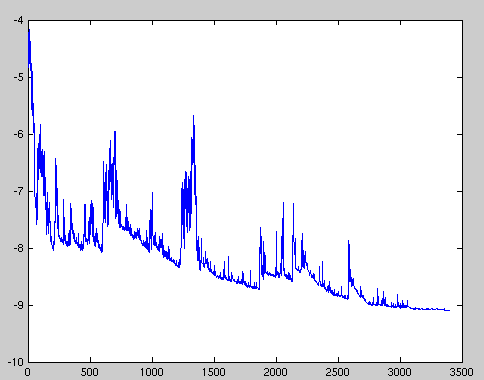
\includegraphics[width=\textwidth]{figures/sgd_fluctuation.png}
\scriptsize{SGD fluctuation - Fonte: \cite{ruder2017}}

\begin{itemize}
    \item SGD realiza atualizações com alta variância
    \item A função objetivo flutua fortemente
    \item Permite escape de mínimos locais, mas complica a convergência
\end{itemize}
\end{column}

\begin{column}{0.48\textwidth}
\begin{itemize}
    \item \textbf{Limitações principais:} \pause
    \begin{itemize}
        \item Alta variância nas atualizações \pause
        \item Progresso lento em ravinas (áreas com curvatura diferente) \pause
        \item Escolha da taxa de aprendizado é crítica \pause
        \item Mesma taxa para todos os parâmetros \pause
        \item Dificuldade em pontos de sela
    \end{itemize} \pause
    \item Estas limitações motivaram as variantes avançadas do SGD
\end{itemize}
\end{column}
\end{columns}

\vspace{0.3cm}
\begin{alertblock}{Desafio}
Como manter as vantagens do SGD (iterações baratas, escape de mínimos locais) enquanto reduzimos seus problemas (oscilação, convergência lenta)?
\end{alertblock}
\end{frame}

\begin{frame}{SGD com Momentum - Qian, 1999}
\begin{itemize}
    \item Inspiração física: uma bola rolando por uma superfície acumula momento \pause
    \item Introduz uma "memória"~ de direções anteriores: \pause
    \begin{align*}
        v_k &= \gamma v_{k-1} + \alpha_k g_{B_k}(x_k) \\
        x_{k+1} &= x_k - v_k
    \end{align*} \pause
    \item O parâmetro $\gamma$ (tipicamente 0.9) controla a influência do histórico \pause
    \item Vantagens: \pause
    \begin{itemize}
        \item Acelera o progresso em direções consistentes \pause
        \item Reduz oscilações em ravinas \pause
        \item Ajuda a superar pequenos mínimos locais e platôs
    \end{itemize} \pause
    \item Desvantagens: \pause
    \begin{itemize}
        \item Pode ultrapassar o mínimo em fundos de ravinas \pause
        \item Ainda usa a mesma taxa para todos os parâmetros
    \end{itemize}
\end{itemize}
\end{frame}

\begin{frame}{Visualização: SGD vs SGD com Momentum}
\begin{columns}[T]
    \begin{column}{0.48\textwidth}
        \centering
        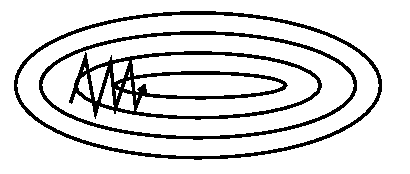
\includegraphics[width=0.9\textwidth]{figures/without_momentum.png}
        
        \small{SGD sem momentum}
    \end{column}
    \begin{column}{0.48\textwidth}
        \centering
        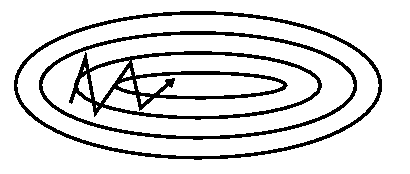
\includegraphics[width=0.9\textwidth]{figures/with_momentum.png}
        
        \small{SGD com momentum}
    \end{column}
\end{columns}

\vspace{0.3cm}
\begin{center}
\small{Comportamento de SGD em ravinas (Fonte: \cite{ruder2017})}
\end{center}

\begin{itemize}
    \item SGD oscila nas encostas enquanto momentum suaviza o caminho
    \item Momentum acelera convergência em direções consistentes
\end{itemize}
\end{frame}


\begin{frame}{Nesterov Accelerated Gradient (NAG) - 1983}
\begin{itemize}
    \item Refinamento do momentum proposto por Yurii Nesterov \pause
    \item Diferença principal: "olha adiante"~ antes de calcular o gradiente \pause
    \begin{align*}
        v_k &= \gamma v_{k-1} + \alpha_k g_{B_k}(x_k - \gamma v_{k-1}) \\
        x_{k+1} &= x_k - v_k
    \end{align*} \pause
    \item O termo $g_{B_k}(x_k - \gamma v_{k-1})$ calcula o gradiente em uma posição antecipada \pause
    \item Vantagens: \pause
    \begin{itemize}
        \item Prevê onde os parâmetros estarão após a aplicação do momentum \pause
        \item Melhor capacidade de desacelerar quando necessário \pause
        \item Convergência teórica melhorada para problemas convexos
    \end{itemize} \pause
    \item Esta simples modificação do momentum proporciona significativas melhorias práticas
\end{itemize}
\end{frame}

\begin{frame}{Visualização: Atualização de Nesterov}
\begin{figure}
\centering
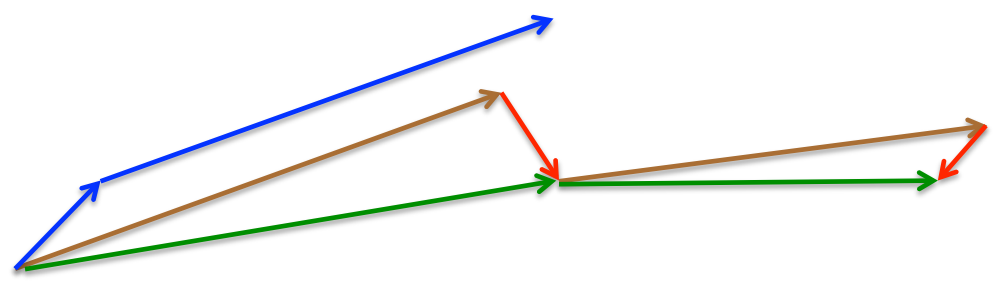
\includegraphics[width=0.4\textwidth]{figures/nesterov_update.png}
\caption{Atualização de Nesterov (Fonte: \cite{ruder2017})}
\end{figure}

\begin{itemize}
    \item Momentum: primeiro calcula o gradiente atual (vetor azul pequeno) e depois dá um grande salto na direção do gradiente acumulado atualizado (vetor azul grande)
    \item NAG: primeiro dá um grande salto na direção do gradiente acumulado anterior (vetor marrom), mede o gradiente e então faz uma correção (vetor verde)
    \item Esta atualização antecipatória impede que avancemos muito rápido e resulta em maior responsividade
\end{itemize}
\end{frame}

\begin{frame}{Adaptive Gradient (Adagrad) - Introdução}
\begin{itemize}
    \item Adagrad (Duchi et al., 2011): adapta as taxas de aprendizado por parâmetro \pause
    \item Princípio: parâmetros que recebem atualizações grandes terão taxas menores \pause
    \item Para cada parâmetro $i$: \pause
    \begin{equation*}
        x_i^{k+1} = x_i^k - \frac{\alpha}{\sqrt{G_{i,i}^k + \epsilon}} g_{B_k,i}(x^k)
    \end{equation*}
    onde $G_{i,i}^k = \sum_{j=1}^{k} (g_{B_j,i}(x^j))^2$ acumula os gradientes ao quadrado \pause
    \item Vantagens: \pause
    \begin{itemize}
        \item Elimina a necessidade de ajuste manual da taxa de aprendizado \pause
        \item Funciona bem com dados esparsos (Natural Language Processing (NLP), visão computacional) \pause
        \item Taxas diferentes para cada parâmetro
    \end{itemize}
\end{itemize}
\end{frame}

\begin{frame}{Adaptive Gradient (Adagrad) - Limitações}
    \begin{itemize}
        \item O acúmulo de gradientes ao quadrado no denominador:
        \pause
        \begin{itemize}
            \item Se os gradientes forem grandes nas iterações iniciais, $G_{k}$ cresce rapidamente
            \pause
            \item Reduz excessivamente a taxa de aprendizado
            \pause
            \item Torna a convergência muito lenta nas fases posteriores
        \end{itemize}
        \pause
        \item Devido a essas limitações, variantes como RMSProp e Adam se tornaram mais populares
    \end{itemize}
\end{frame}

\begin{frame}{Root Mean Square Propagation (RMSprop)}
\begin{itemize}
    \item Introduzido por Geoff Hinton em uma aula de Coursera (não publicado
formalmente)
    \item Modifica o Adagrad para resolver o problema de diminuição excessiva \pause
    \item Substitui a soma acumulada por uma média móvel exponencial: \pause
    \begin{align*}
        v_i^k &= \beta v_i^{k-1} + (1-\beta) (g_{B_k,i}(x^k))^2 \\
        x_i^{k+1} &= x_i^k - \frac{\alpha}{\sqrt{v_i^k + \epsilon}} g_{B_k,i}(x^k)
    \end{align*} \pause
    \item O parâmetro $\beta$ (tipicamente 0.9) controla o decaimento da média \pause
    \item Vantagens: \pause
    \begin{itemize}
        \item "Esquece"~ gradualmente os gradientes antigos \pause
        \item Mantém a adaptabilidade mesmo após muitas iterações \pause
    \end{itemize} \pause
    \item Um dos métodos mais populares para treino de redes neurais
\end{itemize}
\end{frame}

\begin{frame}{Adaptive Moment Estimation (Adam) - Kingma \& Ba, 2015}
\begin{itemize}
    \item Combina as ideias de Momentum e RMSProp \pause
    \item Mantém duas médias móveis:
    \begin{align*}
        m_k &= \beta_1 m_{k-1} + (1 - \beta_1) g_{B_k}(x^k) \quad \text{(primeiro momento)} \\
        v_k &= \beta_2 v_{k-1} + (1 - \beta_2) (g_{B_k}(x^k))^2 \quad \text{(segundo momento)}
    \end{align*} \pause
    \item Corrige o viés inicial das estimativas:
    \begin{align*}
        \hat{m}_k &= \frac{m_k}{1 - \beta_1^k} \quad \text{e} \quad \hat{v}_k = \frac{v_k}{1 - \beta_2^k}
    \end{align*} \pause
    \item Atualização dos parâmetros:
    \begin{equation*}
        x^{k+1} = x^k - \frac{\alpha \hat{m}_k}{\sqrt{\hat{v}_k} + \epsilon}
    \end{equation*}
\end{itemize}
\end{frame}

\begin{frame}{Vantagens e Configuração do Adam}
\begin{itemize}
    \item Principais vantagens do Adam: \pause
    \begin{itemize}
        \item Combina os benefícios do momentum (direção) e adaptação de taxa \pause
        \item Robusto a escolhas de hiperparâmetros (funciona bem com valores default) \pause
        \item Eficaz em problemas de grande escala com muitos parâmetros \pause
        \item Lida bem com gradientes ruidosos e não-estacionários
    \end{itemize} \pause
    \item Valores padrão recomendados: \pause
    \begin{itemize}
        \item $\alpha$ (taxa de aprendizado): 0.001 \pause
        \item $\beta_1$ (decaimento do primeiro momento): 0.9 \pause
        \item $\beta_2$ (decaimento do segundo momento): 0.999 \pause
        \item $\epsilon$ (termo de estabilidade numérica): $10^{-8}$
    \end{itemize} \pause
    \item Na prática, geralmente só é necessário ajustar $\alpha$
\end{itemize}
\end{frame}

\begin{frame}{Outras Variantes Importantes}
\begin{itemize}
    \item Adadelta (Zeiler, 2012) \pause
    \begin{itemize}
        \item Extensão do Adagrad que reduz a diminuição monotônica da taxa \pause
        \item Não requer definição de taxa de aprendizado inicial \pause
        \item Usa apenas informação local para adaptação
    \end{itemize} \pause
    \item AdamW (Loshchilov \& Hutter, 2019) \pause
    \begin{itemize}
        % \item Corrige a implementação da regularização L2 (weight decay) no Adam \pause
        \item Melhora significativamente a generalização em redes neurais
    \end{itemize} \pause
    \item AMSGrad (Reddi et al., 2018) \pause
    \begin{itemize}
        \item Resolve problemas de convergência do Adam em alguns cenários \pause
        \item Usa o máximo dos segundos momentos passados
    \end{itemize} \pause
    \item Nadam (Dozat, 2016) \pause
    \begin{itemize}
        \item Combina Adam com o momentum de Nesterov
    \end{itemize} \pause
    % \item RAdam (Liu et al., 2020) \pause
    % \begin{itemize}
    %     \item Adiciona uma fase de aquecimento (warmup) adaptativa ao Adam \pause
    %     \item Visa resolver a instabilidade inicial em treinamento
    % \end{itemize}
\end{itemize}
\end{frame}

\begin{frame}{Visualização: Comportamento dos Otimizadores}
\begin{figure}
\centering
\animategraphics[width=0.5\textwidth,autoplay,loop,controls]{12}{figures/optimization-on-loss-surface-contours/fig_}{001}{199}
\caption{SGD optimization on loss surface contours}
\end{figure}
\end{frame}

\begin{frame}{Visualização: Comportamento dos Otimizadores}
\begin{figure}
\centering
\animategraphics[width=0.5\textwidth,autoplay,loop,controls]{12}{figures/optimization-on-saddle-point/fig_}{001}{199}
\caption{SGD optimization on saddle point}
\end{figure}
\end{frame}

% \section{Estratégias de Mini-batch}

% \begin{frame}{Importância da Seleção de Mini-batch}
% \begin{itemize}
%     \item A escolha de como formar mini-batches é crucial para o desempenho \pause
%     \item Fatores importantes: \pause
%     \begin{itemize}
%         \item Tamanho do mini-batch: equilíbrio entre computação e estocásticidade \pause
%         \item Esquema de amostragem: aleatório, sequencial, estratificado \pause
%         \item Tamanho do mini-batch adaptativo ou fixo \pause
%         \item Representatividade: garantir diversidade nos dados selecionados
%     \end{itemize} \pause
%     \item Impactos na convergência: \pause
%     \begin{itemize}
%         \item Mini-batches grandes: menos ruído, mais computação, menor regularização \pause
%         \item Mini-batches pequenos: mais ruído, menos computação, maior regularização
%     \end{itemize}
% \end{itemize}
% \end{frame}

% \begin{frame}{Estratégias para Seleção de Mini-batch}
% \begin{itemize}
%     \item Amostragem Aleatória Uniforme \pause
%     \begin{itemize}
%         \item Seleciona amostras com igual probabilidade em cada iteração \pause
%         \item Garantia teórica: estimativa não-viesada do gradiente
%     \end{itemize} \pause
%     \item Amostragem Sem Reposição (por época) \pause
%     \begin{itemize}
%         \item Garante que cada amostra é vista exatamente uma vez por época \pause
%         \item Geralmente implementada como uma permutação aleatória dos dados
%     \end{itemize} \pause
%     \item Tamanho Crescente \pause
%     \begin{itemize}
%         \item Começa com mini-batches pequenos e aumenta gradualmente \pause
%         \item Exemplo: Fountoulakis \& Gondzio (2012) \pause
%         \begin{equation*}
%             |B_{k+1}| = \lceil \min \{ 1.1 \cdot |B_k| + 1, M \} \rceil
%         \end{equation*}
%     \end{itemize}
% \end{itemize}
% \end{frame}

% \begin{frame}{Estratégias Avançadas de Mini-batch}
% \begin{itemize}
%     \item Amostragem Estratificada \pause
%     \begin{itemize}
%         \item Divide os dados em estratos e seleciona proporcionalmente de cada um \pause
%         \item Garante representatividade de classes ou características importantes
%     \end{itemize} \pause
%     \item Amostragem Baseada em Importância \pause
%     \begin{itemize}
%         \item Seleciona amostras com probabilidade proporcional à sua importância \pause
%         \item Importância pode ser baseada no erro, gradiente, ou outra métrica
%     \end{itemize} \pause
%     \item Grupo de Controle (van Herwaarden et al., 2020) \pause
%     \begin{itemize}
%         \item Mantém um subconjunto fixo de amostras "âncora" entre mini-batches \pause
%         \item Reduz a variância e estabiliza a convergência
%     \end{itemize} \pause
%     \item Currículos de Aprendizado \pause
%     \begin{itemize}
%         \item Ordena os exemplos do mais fácil para o mais difícil \pause
%         \item Introduz gradualmente exemplos mais complexos
%     \end{itemize}
% \end{itemize}
% \end{frame}

% \section{Aplicações em Full Waveform Inversion (FWI)}

% \begin{frame}{Introdução ao FWI}
% \begin{itemize}
%     \item Full Waveform Inversion: técnica para recuperar modelos de subsuperfície \pause
%     \item Objetivo: minimizar a diferença entre dados sísmicos observados e simulados \pause
%     \item Formulação como problema de otimização: \pause
%     \begin{equation*}
%         \min_m \sum_{s=1}^{n_s} \sum_{r=1}^{n_r} \| d_{obs}(s,r) - d_{pred}(m,s,r) \|^2
%     \end{equation*}
%     onde $m$ é o modelo, $s$ indexa fontes, $r$ indexa receptores \pause
%     \item Características: \pause
%     \begin{itemize}
%         \item Altamente não-linear e mal-posto \pause
%         \item Computacionalmente intensivo (simulações de onda) \pause
%         \item Grande quantidade de dados (fontes e receptores) \pause
%         \item Múltiplos mínimos locais (problema multi-escala)
%     \end{itemize}
% \end{itemize}
% \end{frame}

% \begin{frame}{Métodos Estocásticos em FWI}
% \begin{itemize}
%     \item Abordagem tradicional: usar todas as fontes em cada iteração \pause
%     \item Abordagem estocástica: selecionar subconjunto de fontes por iteração \pause
%     \item Benefícios: \pause
%     \begin{itemize}
%         \item Redução significativa do custo computacional \pause
%         \item Possibilidade de escape de mínimos locais \pause
%         \item Melhor escalabilidade para grandes conjuntos de dados
%     \end{itemize} \pause
%     \item Desafios específicos: \pause
%     \begin{itemize}
%         \item Alta variabilidade entre gradientes de diferentes fontes \pause
%         \item Informação espacial desigual (fontes não são i.i.d.) \pause
%         \item Tratamento de múltiplas escalas de frequência
%     \end{itemize}
% \end{itemize}
% \end{frame}

% \begin{frame}{Estratégias de Mini-batch para FWI}
% \begin{itemize}
%     \item Considerações específicas para seleção de fontes em FWI: \pause
%     \begin{itemize}
%         \item Distribuição espacial das fontes \pause
%         \item Cobertura angular (azimutes diferentes) \pause
%         \item Conteúdo de frequência dos dados
%     \end{itemize} \pause
%     \item Yang et al. (2018): Amostragem Estratificada de Fontes \pause
%     \begin{itemize}
%         \item Primeira fonte selecionada aleatoriamente \pause
%         \item Demais fontes selecionadas com espaçamento uniforme \pause
%         \item Garante melhor cobertura espacial
%     \end{itemize} \pause
%     \item van Herwaarden et al. (2020): Grupo de Controle \pause
%     \begin{itemize}
%         \item Identifica fontes "influentes" e as mantém entre iterações \pause
%         \item Reduz oscilações na convergência
%     \end{itemize}
% \end{itemize}
% \end{frame}

% \begin{frame}{Evidências Empíricas e Resultados}
% \begin{itemize}
%     \item Estudos comparativos (Richardson, 2018; Sun et al., 2019; Wang et al., 2021): \pause
%     \begin{itemize}
%         \item Adam geralmente supera métodos convencionais em FWI \pause
%         \item Especialmente eficaz com gradientes altamente variáveis \pause
%         \item Menos sensível à escolha de taxa de aprendizado \pause
%         \item Melhor desempenho com conjunto limitado de fontes
%     \end{itemize} \pause
%     \item Estratégias de mini-batch adequadas são cruciais: \pause
%     \begin{itemize}
%         \item Tamanho crescente de mini-batch melhora estabilidade \pause
%         \item Seleção estratificada fornece melhor cobertura espacial \pause
%         \item Grupos de controle reduzem variância sem perder estocásticidade
%     \end{itemize} \pause
%     \item Ganhos típicos: redução de 5-10x no tempo computacional com qualidade comparável
% \end{itemize}
% \end{frame}

\section{Comparação e Recomendações Práticas}

\begin{frame}{Comparação entre Métodos}
\small
\begin{tabular}{|p{2cm}|p{8cm}|}
\hline
\textbf{Método} & \textbf{Características} \\
\hline
SGD simples & Base para outros métodos; alta variância; sensível à taxa de aprendizado; progresso lento em ravinas \\
\hline
Momentum & Acelera convergência em direções consistentes; reduz oscilações; pode ultrapassar mínimos \\
\hline
NAG & Momentum com "olhar adiante"; melhor resposta a mudanças; previne ultrapassagem \\
\hline
Adagrad & Taxas adaptativas por parâmetro; bom para dados esparsos; a taxa diminui excessivamente com o tempo \\
\hline
RMSProp & Corrige Adagrad com média móvel; mantém adaptabilidade ao longo do treinamento \\
\hline
Adam & Combina momentum com adaptação de taxa; correção de viés; robusto a hiperparâmetros \\
\hline
\end{tabular}
\end{frame}

\begin{frame}{Como Escolher o Método Adequado}
\begin{itemize}
    \item Características do problema: \pause
    \begin{itemize}
        \item Tamanho do conjunto de dados \pause
        \item Número de parâmetros \pause
        \item Convexidade/não-convexidade \pause
        \item Esparsidade dos dados \pause
        \item Ruído nos gradientes
    \end{itemize} \pause
    \item Recomendações gerais: \pause
    \begin{itemize}
        \item Problemas convexos simples: SGD com momentum pode ser suficiente \pause
        \item Dados esparsos: métodos adaptativos (Adagrad, RMSProp, Adam) \pause
        \item Deep learning: Adam é geralmente a melhor escolha inicial \pause
        \item FWI: Adam com estratégias de mini-batch específicas \pause
        \item Poucos dados: métodos com regularização L2 explícita (SGD+L2, AdamW)
    \end{itemize}
\end{itemize}
\end{frame}

% \begin{frame}{Questões Práticas de Implementação}
% \begin{itemize}
%     \item Taxa de aprendizado: \pause
%     \begin{itemize}
%         \item Crucial para o desempenho de todos os métodos \pause
%         \item Estratégias de agendamento: constante, decaimento, cíclica, warmup \pause
%         \item Busca em escala logarítmica: testar $10^{-1}, 10^{-2}, 10^{-3}, 10^{-4}$
%     \end{itemize} \pause
%     \item Inicialização: \pause
%     \begin{itemize}
%         \item Médias móveis inicializadas como zero \pause
%         \item Inicialização dos parâmetros: Xavier/Glorot, He, etc.
%     \end{itemize} \pause
%     \item Critérios de parada: \pause
%     \begin{itemize}
%         \item Número fixo de épocas/iterações \pause
%         \item Validação cruzada (early stopping) \pause
%         \item Plateau na função objetivo (com média móvel)
%     \end{itemize}
% \end{itemize}
% \end{frame}

% \begin{frame}{Implementação e Ferramentas}
% \begin{itemize}
%     \item Bibliotecas que implementam métodos estocásticos: \pause
%     \begin{itemize}
%         \item Python: PyTorch, TensorFlow, JAX, scikit-learn \pause
%         \item MATLAB: Statistics and Machine Learning Toolbox \pause
%         \item Julia: Flux.jl, Optim.jl, JUDI (para FWI) \pause
%         \item R: Caret, Torch
%     \end{itemize} \pause
%     \item Considerações de implementação para FWI: \pause
%     \begin{itemize}
%         \item Eficiência na computação do gradiente estocástico \pause
%         \item Gerenciamento de memória para grandes modelos \pause
%         \item Processamento paralelo de diferentes fontes \pause
%         \item Incorporação com simuladores de ondas existentes
%     \end{itemize}
% \end{itemize}
% \end{frame}

% \section{Conclusões e Tendências Futuras}

% \begin{frame}{Recapitulação}
% \begin{itemize}
%     \item Métodos estocásticos são fundamentais para otimização em larga escala \pause
%     \item Evolução: SGD → Momentum → NAG → Métodos Adaptativos \pause
%     \item Cada método aborda limitações específicas dos anteriores \pause
%     \item A escolha de mini-batches é tão importante quanto o algoritmo \pause
%     \item Em FWI: \pause
%     \begin{itemize}
%         \item Redução significativa de custos computacionais \pause
%         \item Melhor escape de mínimos locais \pause
%         \item A escolha adequada do método é crucial para o sucesso
%     \end{itemize}
% \end{itemize}
% \end{frame}

% \begin{frame}{Tendências e Desenvolvimentos Recentes}
% \begin{itemize}
%     \item Adaptação automática de hiperparâmetros \pause
%     \begin{itemize}
%         \item Métodos que ajustam automaticamente taxas de aprendizado \pause
%         \item Estratégias de meta-aprendizado (learning to learn)
%     \end{itemize} \pause
%     \item Otimizadores de segunda ordem e quasi-Newton estocásticos \pause
%     \begin{itemize}
%         \item L-BFGS estocástico \pause
%         \item Métodos de Gauss-Newton aproximados \pause
%         \item Propagação natural estocástica
%     \end{itemize} \pause
%     \item Métodos distribuídos e paralelos \pause
%     \begin{itemize}
%         \item Treinamento distribuído em múltiplos dispositivos \pause
%         \item Agregação eficiente de gradientes \pause
%         \item Técnicas de redução de comunicação
%     \end{itemize} \pause
%     \item Incorporação de informação da curvatura em métodos de primeira ordem
% \end{itemize}
% \end{frame}

% \begin{frame}{Direções de Pesquisa em FWI}
% \begin{itemize}
%     \item Avanços específicos para Full Waveform Inversion: \pause
%     \begin{itemize}
%         \item Métodos multi-escala estocásticos (frequência progressiva) \pause
%         \item Técnicas de amostragem de fontes baseadas em teoria de informação \pause
%         \item Integração com redes neurais para melhorar inicialização do modelo \pause
%         \item Abordagens hibridas: métodos estocásticos + determinísticos
%     \end{itemize} \pause
%     \item Desafios a serem superados: \pause
%     \begin{itemize}
%         \item Lidar com fortes não-linearidades em altas frequências \pause
%         \item Melhorar a convergência em modelos geológicos complexos \pause
%         \item Quantificação de incertezas em resultados de inversão \pause
%         \item Redução da dependência de modelos iniciais precisos
%     \end{itemize}
% \end{itemize}
% \end{frame}

% \begin{frame}{Considerações Finais}
% \begin{itemize}
%     \item Métodos de otimização estocástica representam uma ferramenta fundamental para problemas de larga escala \pause
%     \item Evolução constante de algoritmos, impulsionada por: \pause
%     \begin{itemize}
%         \item Desafios crescentes em aprendizado profundo \pause
%         \item Necessidade de processar quantidades cada vez maiores de dados \pause
%         \item Aplicações em novas áreas, como geofísica e inversão de dados
%     \end{itemize} \pause
%     \item A escolha do método deve considerar: \pause
%     \begin{itemize}
%         \item Características específicas do problema \pause
%         \item Restrições computacionais disponíveis \pause
%         \item Necessidade de precisão vs. velocidade
%     \end{itemize} \pause
%     \item Campo em rápida evolução - importância de acompanhar a literatura recente
% \end{itemize}
% \end{frame}

\begin{frame}{Agradecimento e Referências}
\begin{center}
\Large{Obrigado pela atenção!}

\vspace{1em}
\normalsize{Perguntas?}
\end{center}

\vspace{1em}
\small
\begin{thebibliography}{9}
    \bibitem{robbins1951} Robbins, H., \& Monro, S. (1951). A stochastic approximation method. The annals of mathematical statistics, 400-407.
    \bibitem{kingma2015} Kingma, D. P., \& Ba, J. (2015). Adam: A method for stochastic optimization. ICLR.
    \bibitem{duchi2011} Duchi, J., Hazan, E., \& Singer, Y. (2011). Adaptive subgradient methods for online learning and stochastic optimization. JMLR.
    \bibitem{richardson2018} Richardson, A. (2018). Seismic Full-Waveform Inversion Using Deep Learning Tools and Techniques. arXiv preprint.
    \bibitem{van2020} van Herwaarden et al. (2020). Stochastic amplitude versus offset inversion with mini-batches. Geophysics.
    \bibitem{friedlander2012} Friedlander, M. P., \& Schmidt, M. (2012). Hybrid Deterministic-Stochastic Methods for Data Fitting. SIAM Journal on Scientific Computing, 34(3), A1380-A1405. doi:10.1137/110830629
    \bibitem{ruder2017} Ruder, S. (2017). An overview of gradient descent optimization algorithms. arXiv preprint arXiv:1609.04747.
\end{thebibliography}
\end{frame}

\end{document}